\documentclass[12pt]{article}

\usepackage{caption}
\usepackage{subcaption}
\usepackage{float}
\usepackage{makecell}
\usepackage{amsmath}
\usepackage{graphicx}
\graphicspath{ {./images/} }
\usepackage[utf8]{inputenc}
\usepackage[russian]{babel}
\usepackage{geometry}
 \geometry{
 a4paper,
 left=20mm,
 right=20mm,
 top=20mm,
 bot=20mm,
 }

\begin{document}

\begin{titlepage}
\begin{center}
    {\small НАЦИОНАЛЬНЫЙ ИССЛЕДОВАТЕЛЬСКИЙ УНИВЕРСИТЕТ ИТМО} \\
    {\small Факультет систем управления и робототехники} \\
    \vspace*{10\baselineskip}
    {\LARGEМоделирование динамических систем} \\
    \ \\
    {\LARGEЛабораторная работа №3} \\
    \ \\
    {\LARGEБифуркации} \\
    \ \\
    Вариант 2 \\
    \vspace*{10\baselineskip}
    \hfill {\small Выполнил студент:} \\
    \hfill {\small Кирбаба Д.Д. R3338} \\
    \ \\
    \hfill {\small Преподаватель:} \\
    \hfill {\small Семенов Д.М.} \\
    \mbox{}
    \vfill {\smallг. Санкт-Петербург\\2023}
\end{center}
\end{titlepage}

\section*{Задание 1}
Дана следующая нелинейная система:
\[
\begin{cases}
    \dot{x_1} = -x_1\\
    \dot{x_2} = r x_2 + x_2^3 - x_2^5
\end{cases}
\]\\
Необходимо найти все возможные бифуркации в системе. Определить тип точек равновесия для каждых возможных значений бифуркационного параметра $r$.\\
Также требуется отобразить фазовые портреты линеаризованной и исходной нелинейной систем для каждого типа точек равновесия.\\
\ \\
Для начала, найдем точки равновесия системы.\\
Для их поиска, необходимо приравнять левую часть (производные) к нулю и решить систему:
\[
\begin{cases}
    -x_1 = 0\\
    r x_2 + x_2^3 - x_2^5 = 0
\end{cases}
\Rightarrow
\begin{cases}
    x_1^* = 0\\
    x_2^* = 0
\end{cases}, \ if \ r \geq - \frac{1}{4}: \
\begin{cases}
    x_1^* = 0\\
    x_2^* = \pm \frac{\sqrt{1 \pm \sqrt{4r+1}}}{\sqrt{2}}
\end{cases}
\]\\
Итого, имеем единственную точку равновесия $(x_1^*=0,\ x_2^*=0)$, если $r < - \frac{1}{4}$. \\
\ \\
Имеем три точки равновесия $(x_1^*=0,\ x_2^*=0), \ (x_1^*=0,\ x_2^*=\pm \frac{1}{\sqrt{2}})$, если $r=-\frac{1}{4}$.\\
\ \\
Имеем пять точек равновесия $(x_1^*=0,\ x_2^*=0), (x_1^*=0,\ x_2^*=\pm \frac{\sqrt{1 \pm \sqrt{4r+1}}}{\sqrt{2}})$, если $r \in (- \frac{1}{4},\ 0)$.\\
\ \\
Имеем три точки равновесия $(x_1^*=0,\ x_2^*=0), (x_1^*=0,\ x_2^*=\pm 1)$, если $r=0$.\\
\ \\
Имеем три точки равновесия $(x_1^*=0,\ x_2^*=0), (x_1^*=0,\ x_2^*=\pm \frac{\sqrt{1 + \sqrt{4r+1}}}{\sqrt{2}})$, если $r>0$.\\
\ \\
Составим матрицу Якоби системы:
\[
    A = \begin{bmatrix}
\frac{\delta f_1(x_1,\ x_2)}{\delta x_1} & \frac{\delta f_1(x_1,\ x_2)}{\delta x_2}\\
\frac{\delta f_2(x_1,\ x_2)}{\delta x_1} & \frac{\delta f_2(x_1,\ x_2)}{\delta x_2}
\end{bmatrix} = 
\begin{bmatrix}
-1 & 0\\
0 & r + 3x_2^2 - 5x_2^4
\end{bmatrix}
\]
Рассмотрим точки равновесия $x_2 = \{ 0; \ \frac{\sqrt{1+\sqrt{4r+1}}}{\sqrt{2}}; \ -\frac{\sqrt{1+\sqrt{4r+1}}}{\sqrt{2}}; \ \frac{\sqrt{1-\sqrt{4r+1}}}{\sqrt{2}}; \ -\frac{\sqrt{1-\sqrt{4r+1}}}{\sqrt{2}} \}$:
\[
A_1 = \left.\frac{df(x_2)}{d(x_2)}\right|_{x_{2_1} = 0} = r,
\]
\[
A_2 = \left.\frac{df(x_2)}{d(x_2)}\right|_{x_{2_2} = \frac{\sqrt{1+\sqrt{4r+1}}}{\sqrt{2}}} = -4r - \sqrt{4r+1} - 1,
\]
\[
A_3 = \left.\frac{df(x_2)}{d(x_2)}\right|_{x_{2_3} = -\frac{\sqrt{1+\sqrt{4r+1}}}{\sqrt{2}}} = -4r - \sqrt{4r+1} - 1,
\]
\[
A_4 = \left.\frac{df(x_2)}{d(x_2)}\right|_{x_{2_4} = \frac{\sqrt{1-\sqrt{4r+1}}}{\sqrt{2}}} = -4r + \sqrt{4r+1} - 1,
\]
\[
A_5 = \left.\frac{df(x_2)}{d(x_2)}\right|_{x_{2_5} = -\frac{\sqrt{1-\sqrt{4r+1}}}{\sqrt{2}}} = -4r + \sqrt{4r+1} - 1,
\]
В итоге получаем, что \\
$x_{2_1}^* = 0 \Rightarrow \dot{x_2} = A_1 x_2 = r x_2 \Rightarrow$ устойчиво $\forall r<0$ и неустойчиво $\forall r>0$; \\
\ \\
$x_{2_{2,3}}^* = \pm\frac{\sqrt{1+\sqrt{4r+1}}}{\sqrt{2}} \Rightarrow \dot{x_2} = A_{2,3} x_2 = (-4r - \sqrt{4r+1} - 1)x_2 \Rightarrow$ устойчиво $\forall r>-\frac{1}{4}$; \\
\ \\
$x_{2_{4,5}}^* = \pm\frac{\sqrt{1-\sqrt{4r+1}}}{\sqrt{2}} \Rightarrow \dot{x_2} = A_{4,5} x_2 = (-4r + \sqrt{4r+1} - 1)x_2 \Rightarrow$ устойчиво $\forall r>0$ и неустойчиво $\forall -\frac{1}{4}<r<0$; \\
\ \\
Теперь будем рассматривать целую систему вместе с первым уравнением:
\[
\begin{cases}
    \dot{x_1} = -x_1\\
    \dot{x_2} = r x_2 + x_2^3 - x_2^5
\end{cases}
\]
Итого, имеем:
\begin{center}
\begin{tabular}{ |c|c| } 
 \hline
 $r < -1/4$ & $(0, \ 0)$ - устойчивый узел \\ 
  \hline
 $r = -1/4$ & \makecell{$(0, \ 0)$ - устойчивый узел \\ $(0, \ \pm 1/\sqrt{2})$ - два устойчивых узла со смещением}\\ 
  \hline
 $r \in (-1/4, \ 0)$ & \makecell{$(0, \ 0)$ - устойчивый узел \\ $(0, \ \pm \sqrt{1+\sqrt{4r+1}}/\sqrt{2})$ - два устойчивых узла \\ 
 $(0, \ \pm \sqrt{1-\sqrt{4r+1}}/\sqrt{2})$ - два неустойчивых положения (седла)}} \\ 
  \hline
 $r = 0$ & \makecell{
 $(0, \ 0)$ - устойчивый узел со смещением \\
 $(0, \ \pm 1)$ - два устойчивых узла \\
 } \\
  \hline
 $r > 0$ & \makecell{
 $(0, \ 0)$ - неустойчивый узел (седло) \\
 $(0, \ \pm \sqrt{1+\sqrt{4r+1}}/\sqrt{2})$ - два устойчивых узла \\
 } \\
 \hline
\end{tabular}
\end{center} \\
\ \\
Теперь отобразим фазовые портреты линеаризованной и исходной нелинейной систем для каждого типа точек равновесия. \\

\begin{figure}[H]
     \centering
     \begin{subfigure}[b]{0.3\textwidth}
         \centering
         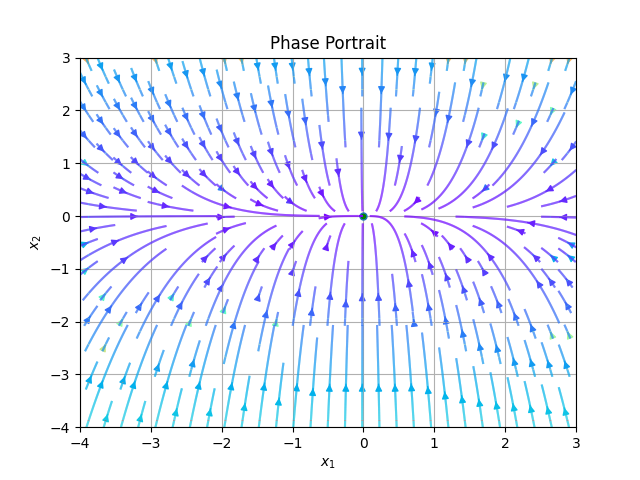
\includegraphics[width=\textwidth]{img_-4.1.png}
         \caption{$r=-4$}
         \label{fig:img_-4.1.png}
     \end{subfigure}
     \hfill
     \begin{subfigure}[b]{0.3\textwidth}
         \centering
         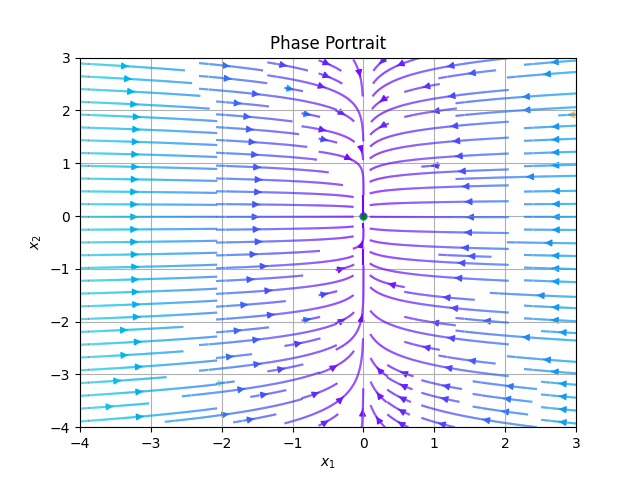
\includegraphics[width=\textwidth]{img_-0.1.png}
         \caption{$r=-0.1$}
         \label{fig:img_-0.1.png}
     \end{subfigure}
     \hfill
     \begin{subfigure}[b]{0.3\textwidth}
         \centering
         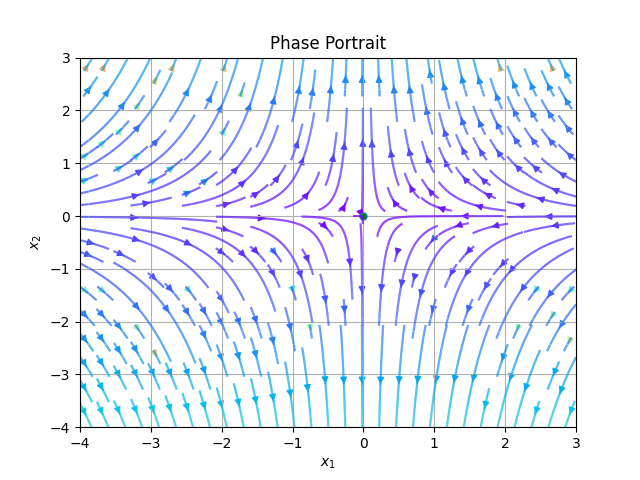
\includegraphics[width=\textwidth]{img_2.9.png}
         \caption{$r=3$}
         \label{fig:img_2.9.png}
     \end{subfigure}
        \caption{Нелинейная система}
        \label{fig:three graphs}
\end{figure}

\begin{center}
    Один устойчивый узел в $(0, \ 0)$ \\
    \downarrow \\
    $(0, \ 0)$ - устойчивый узел, $(0, \ \pm \sqrt{1+\sqrt{4r+1}}/\sqrt{2})$ - два устойчивых узла, 
$(0, \ \pm \sqrt{1-\sqrt{4r+1}}/\sqrt{2})$ - два неустойчивых положения (седла) \\
    \downarrow \\
    $(0, \ 0)$ - неустойчивый узел (седло), $(0, \ \pm \sqrt{1+\sqrt{4r+1}}/\sqrt{2})$ - два устойчивых узла \\
\end{center}

\begin{figure}[H]
     \centering
     \begin{subfigure}[b]{0.3\textwidth}
         \centering
         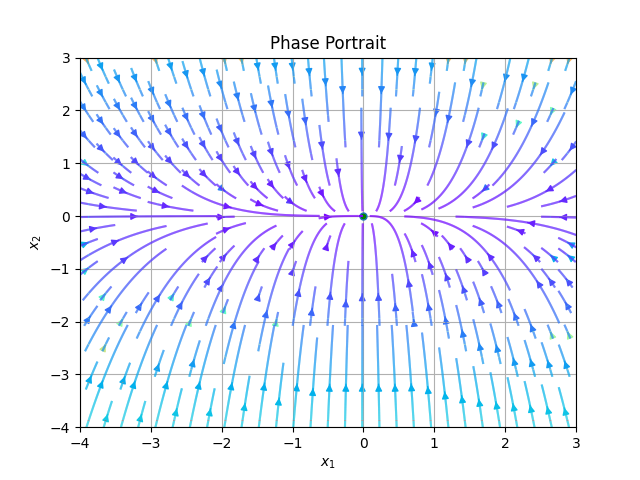
\includegraphics[width=\textwidth]{l_0_0_img_-4.1.png}
         \caption{$r=-4$}
         \label{fig:l_0_0_img_-4.1.png}
     \end{subfigure}
     \hfill
     \begin{subfigure}[b]{0.3\textwidth}
         \centering
         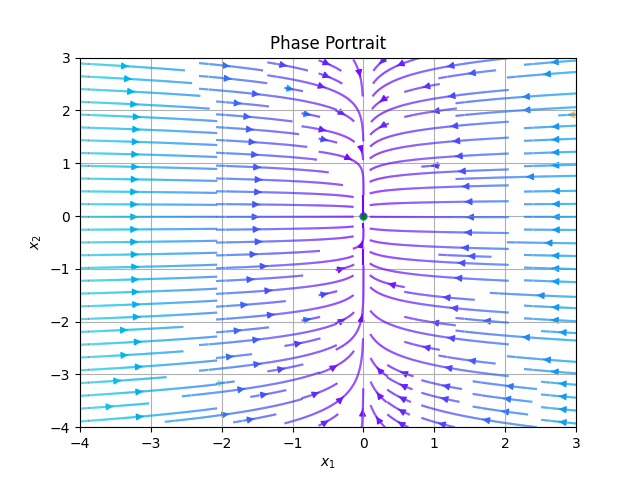
\includegraphics[width=\textwidth]{l_0_0_img_-0.1.png}
         \caption{$r=-0.1$}
         \label{fig:l_0_0_img_-0.1.png}
     \end{subfigure}
     \hfill
     \begin{subfigure}[b]{0.3\textwidth}
         \centering
         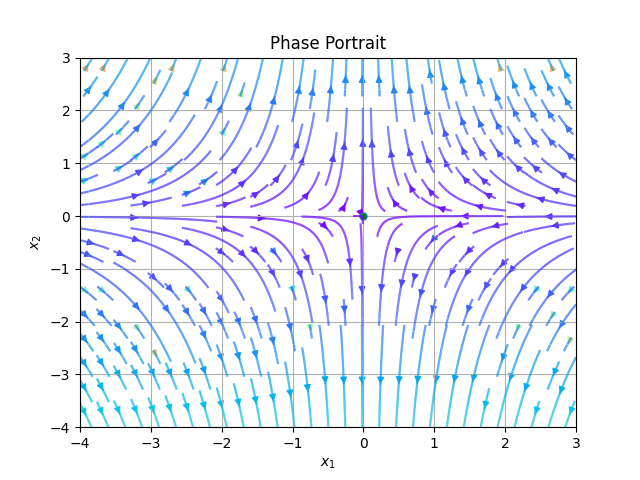
\includegraphics[width=\textwidth]{l_0_0_img_2.9.png}
         \caption{$r=3$}
         \label{fig:l_0_0_img_2.9.png}
     \end{subfigure}
        \caption{Линеаризованная система около $(0,\ 0)$}
        \label{fig:three graphs}
\end{figure}

\begin{center}
    Устойчивый узел \\
    \downarrow \\
    Устойчивый узел \\
    \downarrow \\
    Седло \\
\end{center}

\begin{figure}[H]
     \centering
     \begin{subfigure}[b]{0.3\textwidth}
         \centering
         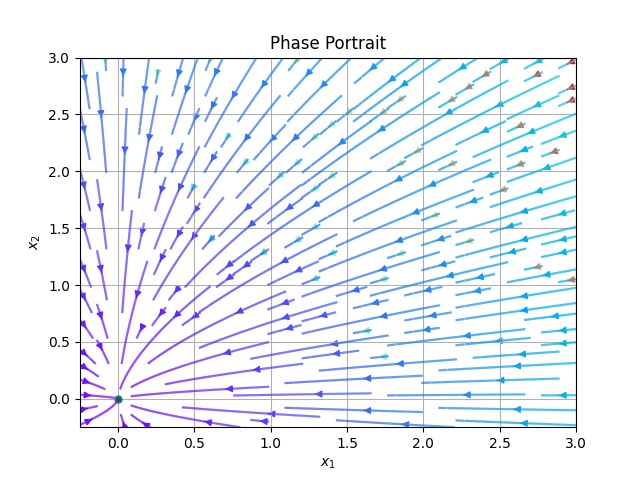
\includegraphics[width=\textwidth]{l_p_p_img_-0.2.png}
         \caption{$r=-1/4$}
         \label{fig:l_p_p_img_-0.2.png}
     \end{subfigure}
     \hfill
     \begin{subfigure}[b]{0.3\textwidth}
         \centering
         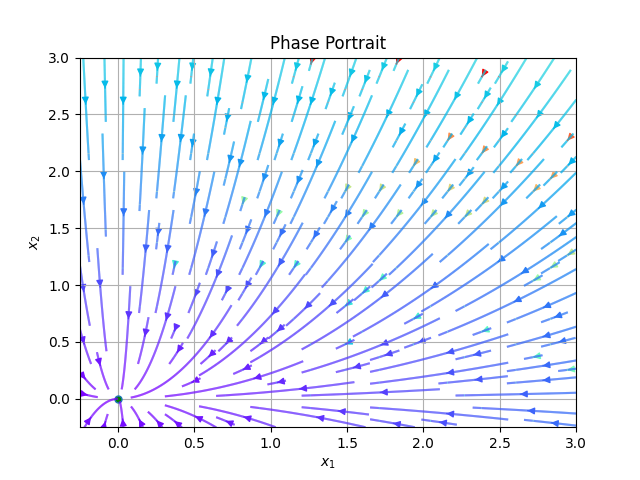
\includegraphics[width=\textwidth]{l_p_p_img_0.0.png}
         \caption{$r=0$}
         \label{fig:l_p_p_img_0.0.png}
     \end{subfigure}
     \hfill
     \begin{subfigure}[b]{0.3\textwidth}
         \centering
         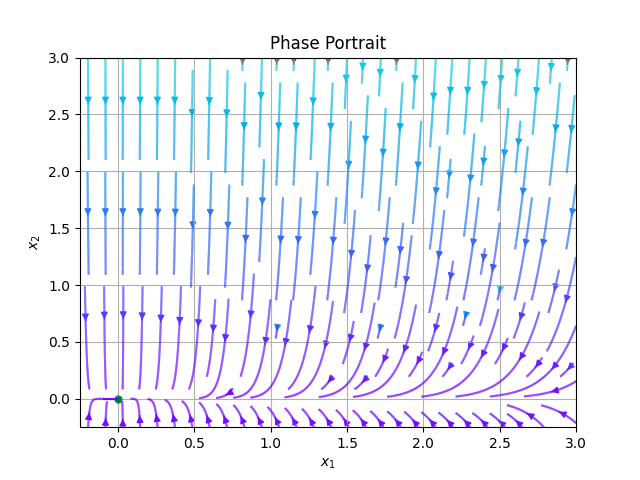
\includegraphics[width=\textwidth]{l_p_p_img_3.0.png}
         \caption{$r=3$}
         \label{fig:l_p_p_img_3.0.png}
     \end{subfigure}
        \caption{Линеаризованная система около $(0,\ \sqrt{1+\sqrt{4r+1}}/\sqrt{2})$}
        \label{fig:three graphs}
\end{figure}

\begin{center}
    Устойчивый узел \\
    \downarrow \\
    Устойчивый узел \\
    \downarrow \\
    Устойчивый узел \\
\end{center}

\begin{figure}[H]
     \centering
     \begin{subfigure}[b]{0.3\textwidth}
         \centering
         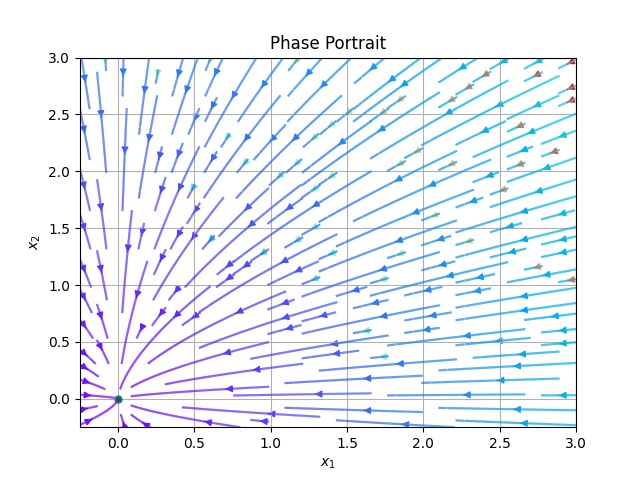
\includegraphics[width=\textwidth]{l_n_p_img_-0.2.png}
         \caption{$r=-1/4$}
         \label{fig:l_n_p_img_-0.2.png}
     \end{subfigure}
     \hfill
     \begin{subfigure}[b]{0.3\textwidth}
         \centering
         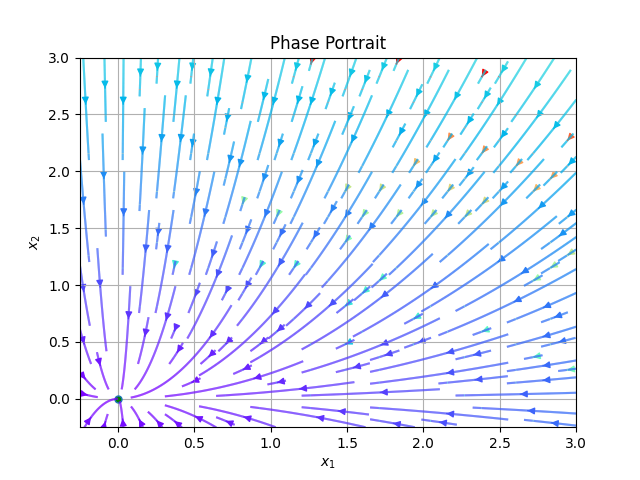
\includegraphics[width=\textwidth]{l_n_p_img_0.0.png}
         \caption{$r=0$}
         \label{fig:l_n_p_img_0.0.png}
     \end{subfigure}
     \hfill
     \begin{subfigure}[b]{0.3\textwidth}
         \centering
         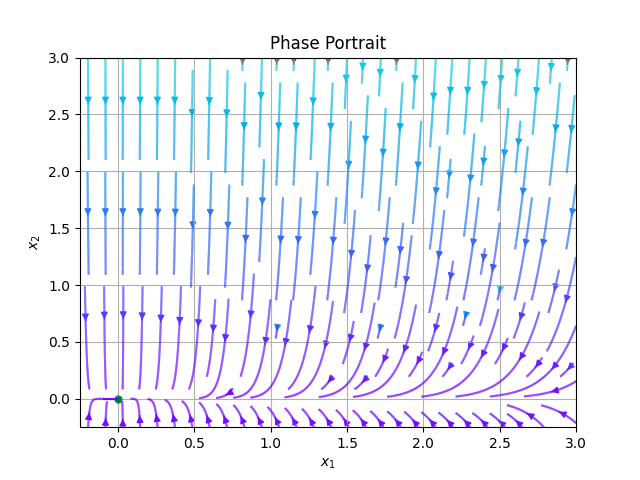
\includegraphics[width=\textwidth]{l_n_p_img_3.0.png}
         \caption{$r=3$}
         \label{fig:l_n_p_img_3.0.png}
     \end{subfigure}
        \caption{Линеаризованная система около $(0,\ -\sqrt{1+\sqrt{4r+1}}/\sqrt{2})$}
        \label{fig:three graphs}
\end{figure}

\begin{center}
    Устойчивый узел \\
    \downarrow \\
    Устойчивый узел \\
    \downarrow \\
    Устойчивый узел \\
\end{center}

\begin{figure}[H]
     \centering
     \begin{subfigure}[b]{0.3\textwidth}
         \centering
         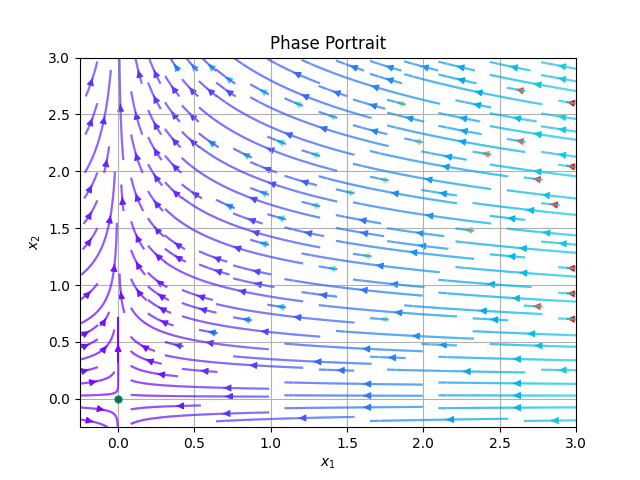
\includegraphics[width=\textwidth]{l_p_n_img_-0.2.png}
         \caption{$r=-1/4$}
         \label{fig:l_p_n_img_-0.2.png}
     \end{subfigure}
     \hfill
     \begin{subfigure}[b]{0.3\textwidth}
         \centering
         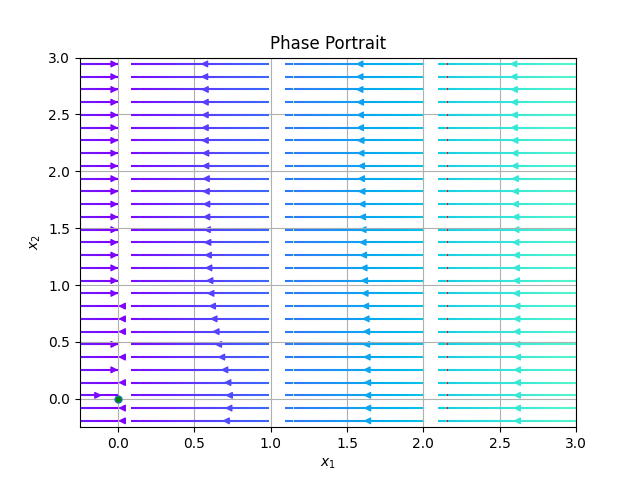
\includegraphics[width=\textwidth]{l_p_n_img_0.0.png}
         \caption{$r=0$}
         \label{fig:l_p_n_img_0.0.png}
     \end{subfigure}
     \hfill
     \begin{subfigure}[b]{0.3\textwidth}
         \centering
         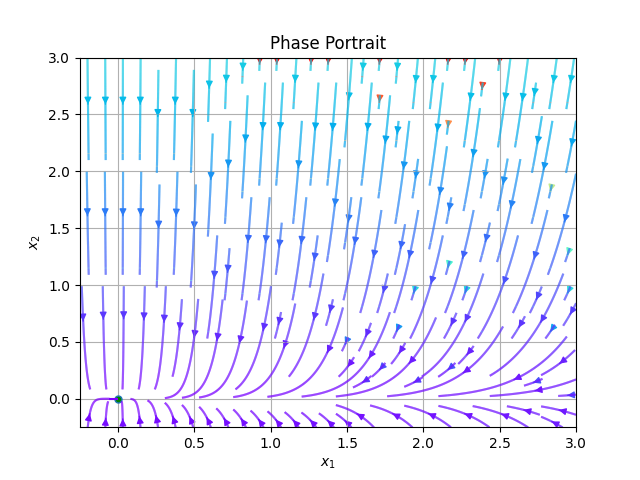
\includegraphics[width=\textwidth]{l_p_n_img_3.0.png}
         \caption{$r=3$}
         \label{fig:l_p_n_img_3.0.png}
     \end{subfigure}
        \caption{Линеаризованная система около $(0,\ \sqrt{1-\sqrt{4r+1}}/\sqrt{2})$}
        \label{fig:three graphs}
\end{figure}

\begin{center}
    Седло \\
    \downarrow \\
    Граница устойчивости \\
    \downarrow \\
    Устойчивый узел \\
\end{center}

\begin{figure}[H]
     \centering
     \begin{subfigure}[b]{0.3\textwidth}
         \centering
         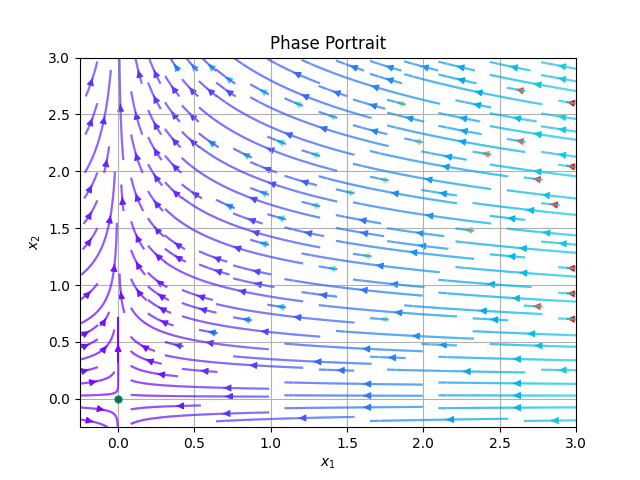
\includegraphics[width=\textwidth]{l_n_n_img_-0.2.png}
         \caption{$r=-1/4$}
         \label{fig:l_n_n_img_-0.2.png}
     \end{subfigure}
     \hfill
     \begin{subfigure}[b]{0.3\textwidth}
         \centering
         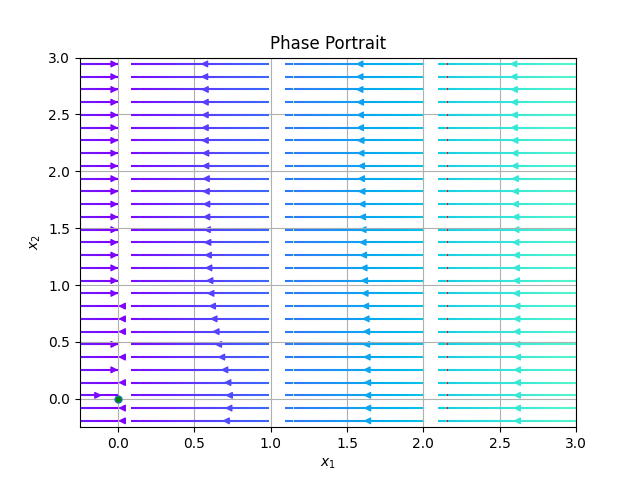
\includegraphics[width=\textwidth]{l_n_n_img_0.0.png}
         \caption{$r=0$}
         \label{fig:l_n_n_img_0.0.png}
     \end{subfigure}
     \hfill
     \begin{subfigure}[b]{0.3\textwidth}
         \centering
         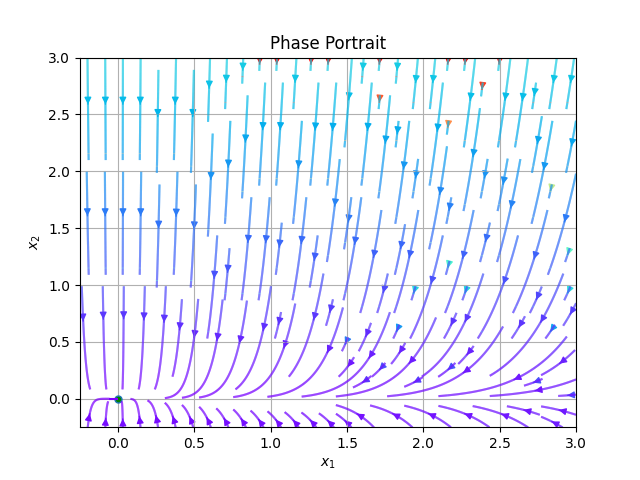
\includegraphics[width=\textwidth]{l_n_n_img_3.0.png}
         \caption{$r=3$}
         \label{fig:l_n_n_img_3.0.png}
     \end{subfigure}
        \caption{Линеаризованная система около $(0,\ -\sqrt{1-\sqrt{4r+1}}/\sqrt{2})$}
        \label{fig:three graphs}
\end{figure}

\begin{center}
    Седло \\
    \downarrow \\
    Граница устойчивости \\
    \downarrow \\
    Устойчивый узел \\
\end{center}

\section*{Выводы}
В данной работе было проведено исследование системы с бифуркационным параметром $r$. Было аналитически предсказано, что поведение системы будет меняться при прохождении бифуркационного параметра порогов $\{-\frac{1}{4}; \ 0\}$. Также были построены фазовые портреты нелинейной и линеаризованной около положений равновесия для наглядной картины преобразования системы при изменении бифуркационного параметра.
\end{document}